%=======================================================================
% NEW SUBSECTION for section 4, to sit after \subsection{Loss to the
% formation and the role of the well field}. It closes the \todo{} on
% "Profiles along the well at CSS".
%
% Figures are the BOREAS analogues of Figs. 5-8 of the IHTC hairpin paper,
% Depth is on the ORDINATE, increasing downward.
%
% COORDINATE WARNING: the solver's z is NOT depth. z = 0 is the BOTTOM of
% the well on charge (the water arrives there down the downcomer), so
% depth = L_well - z. The figures use formation_profile's depth array so
% there is a single definition. Both half-cycle histories come back in the
% CHARGE frame.
%
% An animation of the full cycle is supplied as supplementary material:
% BOREAS_cycle.mp4 (and .gif). It is NOT referenced by a \ref, so it can be
% dropped without touching the text.
%
% boreas.py v1.3, simulate_css_corrected(..., record=True), reference case:
% 1000-well vertical array in double rows on four islands, n_s = 99,
% N_lay = 9, t_ch = t_dc = 10 h.
%
% Labels: fig:prof-T, fig:prof-melt, fig:prof-Ui, fig:prof-int.
%=======================================================================
\subsection{Thermal behaviour along the well}
\label{sec:res-thermal}

In the downcomer geometry each fin tube occupies every depth once, so a
profile along the tube is a profile down the well and the melting staircase
$T_{m,k}$ is fixed in space rather than carried along a folded hairpin. The
figures below are taken from one recorded cycle at cyclic steady state and
are drawn with depth increasing downward, as the well does. An animation of
the same cycle is provided as supplementary material.

\paragraph{The cascade is graded with the rock, and the flow is
counter-current} The hottest layer, $T_{m}=\SI{150}{\celsius}$, is at the
\emph{bottom} of the well and the coolest, \SI{101}{\celsius}, at the top.
That is the right way round: the undisturbed rock runs from
\SI{18}{\celsius} at the surface to \SI{86}{\celsius} at
\SI{1516}{\metre}, so grading the store with the geotherm puts the largest
PCM-to-rock difference where the rock is coldest only at the shallow end,
where the inventory is least hot. The alternative grading would place
\SI{150}{\celsius} material against \SI{18}{\celsius} rock.

Figure~\ref{fig:prof-T} gives the secondary-fluid and PCM temperatures along
the well. During charging the water descends the insulated downcomer without
exchanging, enters the fin tubes at the \emph{bottom} at
$T_\mathrm{4c}=\SI{160}{\celsius}$ and cools as it \emph{rises} through
progressively cooler layers, leaving the tubes near \SI{109}{\celsius}.
During discharging the flow reverses: water returns from the ORC at
$T_\mathrm{3d}=\SI{91.1}{\celsius}$, enters the fin tubes at the \emph{top},
warms as it \emph{descends} toward the hotter layers, and leaves the bottom
between \SI{152}{\celsius} and \SI{124}{\celsius} over the half-cycle before
returning up the downcomer. The insulated downcomer therefore always carries
the hot stream --- in on charge, out on discharge --- which is what it is
for. The cascade is traversed in opposite directions in the two half-cycles,
and that is what allows one staircase to serve both: each layer sees the
fluid on the correct side of its own $T_{m,k}$ in both periods.

The PCM temperature, dashed in Figure~\ref{fig:prof-T}, makes the mechanism
explicit. Within a layer it sits on the melting plateau while phase change
proceeds and bows toward the fluid only once that layer is spent; at a layer
boundary the driving difference is restored and the bow resets. The fluid
profile therefore tracks the staircase down the whole well rather than
decaying smoothly toward it, and the fluid-to-PCM difference stays bounded
instead of collapsing at the far end. This is the mechanism identified for
the hairpin store, and it survives the change of geometry.

\begin{figure}[htbp]
\centering
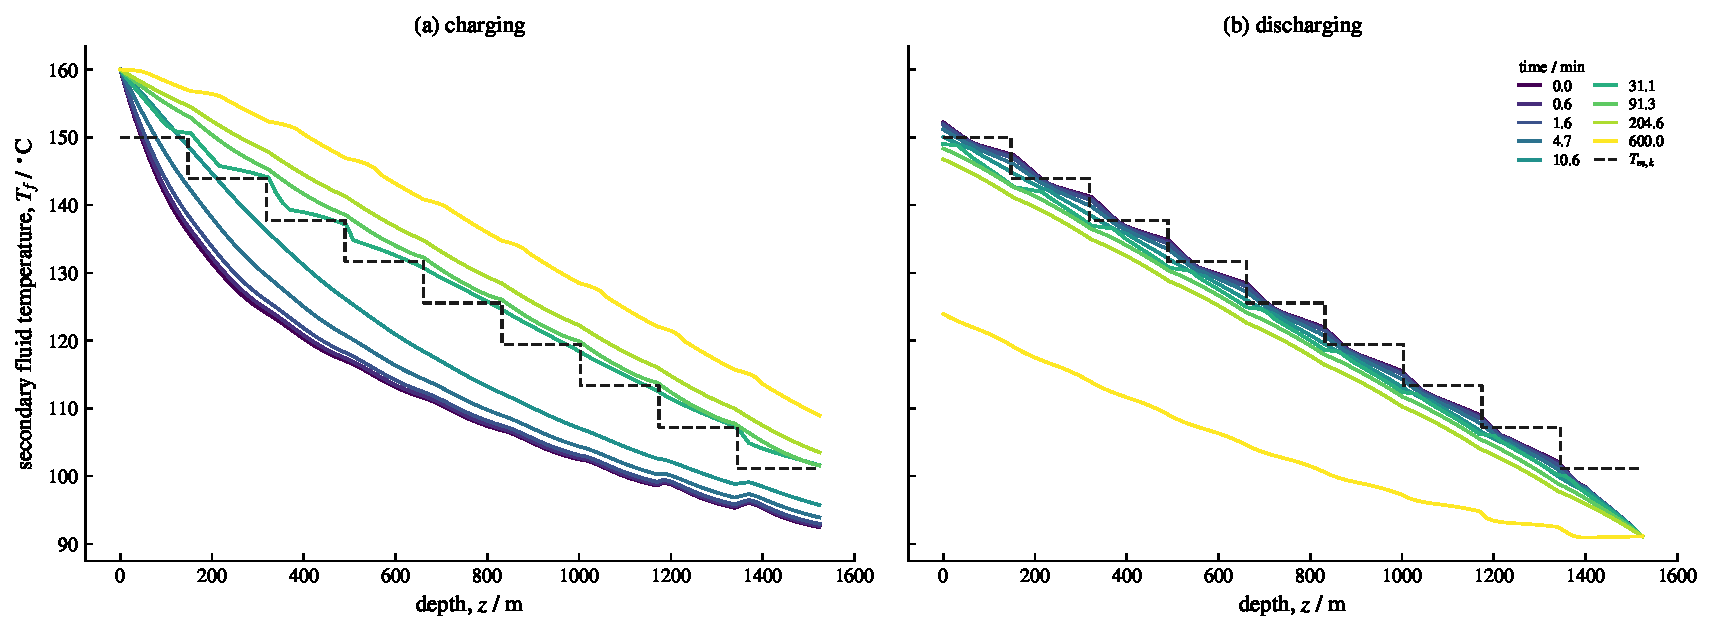
\includegraphics[width=\linewidth]{figures/BOREAS_prof_Tfluid.pdf}
\caption{Secondary-fluid temperature (solid) and PCM temperature (dotted)
along the well during charging and discharging, at cyclic steady state.
Black dashed: the melting staircase $T_{m,k}$, hottest at the bottom.
Curves are labelled by time from the start of the half-cycle. Charging
enters the fin tubes at the bottom and rises; discharging enters at the top
and descends.}
\label{fig:prof-T}
\end{figure}

\paragraph{Phase change is distributed, not concentrated}
Figure~\ref{fig:prof-melt} shows the local melted fraction,
$A_\mathrm{melt}/A_\mathrm{av}$. Within each layer the melted fraction falls
with distance from the layer inlet, as the driving difference is consumed;
at each layer boundary the difference is restored and the melted fraction
jumps back up. The result is the sawtooth, and its significance is that the
envelope is nearly flat: the shallowest and deepest layers reach comparable
melted fractions, where a single-$T_m$ store would melt the first layer
completely and leave the last barely touched. By the end of charging the
volume-averaged melted fraction is $\bar\varepsilon_\mathrm{ch}=0.897$ and by
the end of discharging the store has returned essentially to the solid state,
$\bar\varepsilon_\mathrm{dc}=0.001$, so the cycled fraction is close to the
whole inventory.

\begin{figure}[htbp]
\centering
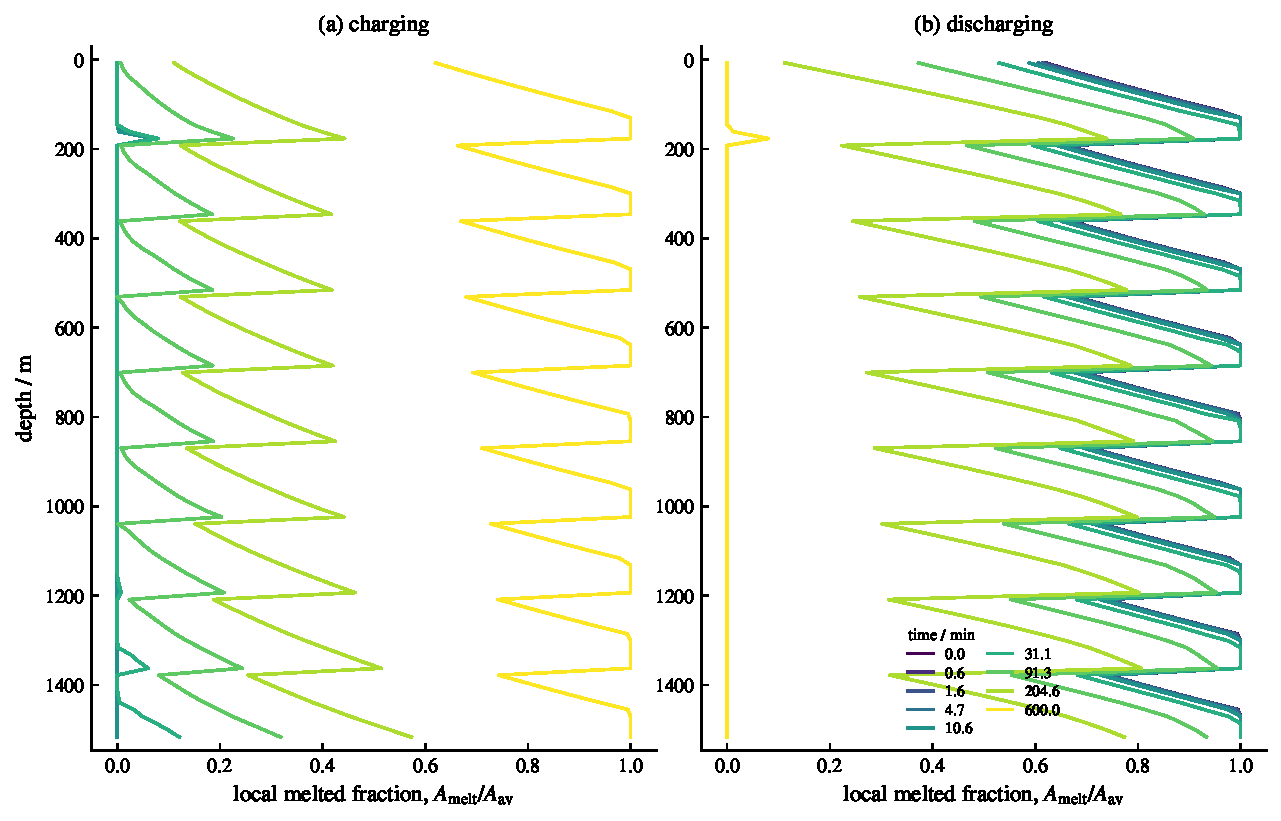
\includegraphics[width=\linewidth]{figures/BOREAS_prof_melt.pdf}
\caption{Local melted fraction of the PCM along the well. Curve legends as
in Figure~\ref{fig:prof-T}. The sawtooth is the layering: the envelope is
far flatter than the decay a single melting temperature would produce.}
\label{fig:prof-melt}
\end{figure}

\paragraph{The overall coefficient follows the phase-change front}
The same pattern appears in the overall heat transfer coefficient referred to
the inner tube area, Figure~\ref{fig:prof-Ui}. $U_i$ ranges from about
\SIrange{74}{781}{\watt\per\meter\squared\per\kelvin} over the cycle. Within
a layer the melted shell thickens with distance from the layer inlet, the
PCM-side resistance grows and $U_i$ falls; at the next layer boundary the
shell is thin again and $U_i$ recovers. Early in each half-cycle, before any
phase change has occurred, $U_i$ is uniform along the well at the value set
by the solid PCM, which is the flat line in each panel.

The local minima should not be read as a defect. A store with a single
melting temperature would show higher $U_i$ near the inlet and a far lower
one at depth, together with the non-uniform melting that
Figure~\ref{fig:prof-melt} rules out; the layered arrangement trades peak
local conductance for uniformity of utilisation along the well.

\begin{figure}[htbp]
\centering
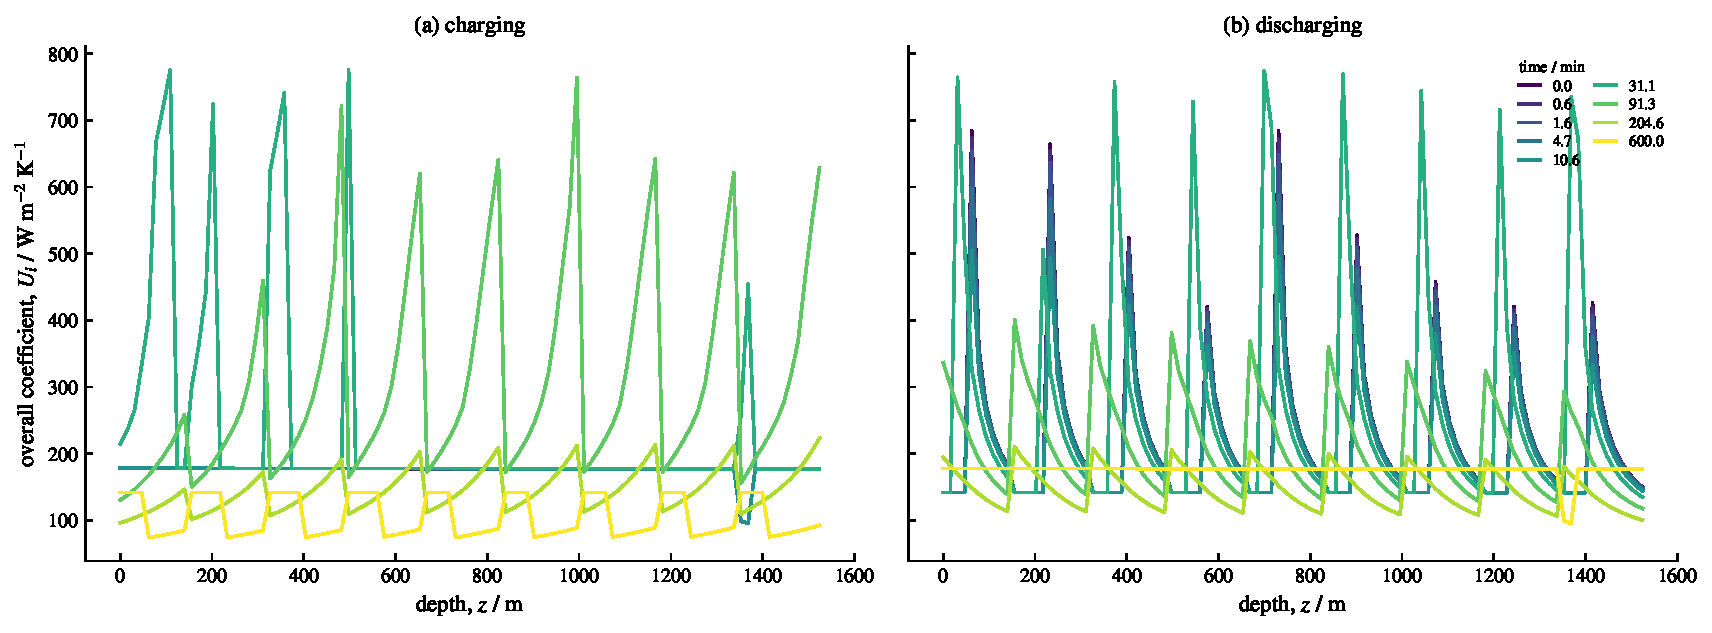
\includegraphics[width=\linewidth]{figures/BOREAS_prof_Ui.pdf}
\caption{Overall heat transfer coefficient on the inner tube area along the
well. Curve legends as in Figure~\ref{fig:prof-T}.}
\label{fig:prof-Ui}
\end{figure}

\paragraph{Integrated behaviour}
Figure~\ref{fig:prof-int} gives the heat transfer rate integrated along the
well, per storage well, together with the volume-averaged melted fraction.
The magnitude of the rate falls through both half-cycles as the phase-change
shell thickens and the PCM-side resistance grows, while the melted fraction
rises on charge and falls on discharge. The charging and discharging rates
are not mirror images: the charge is driven by a larger fluid-to-PCM
difference, so it both melts more and does so faster, which is why the
half-cycles balance at unequal mass flow rates
($\md_\mathrm{ch}=\SI{0.531}{\kilogram\per\second}$ and
$\md_\mathrm{dc}=\SI{0.534}{\kilogram\per\second}$ per fin tube).

\begin{figure}[htbp]
\centering
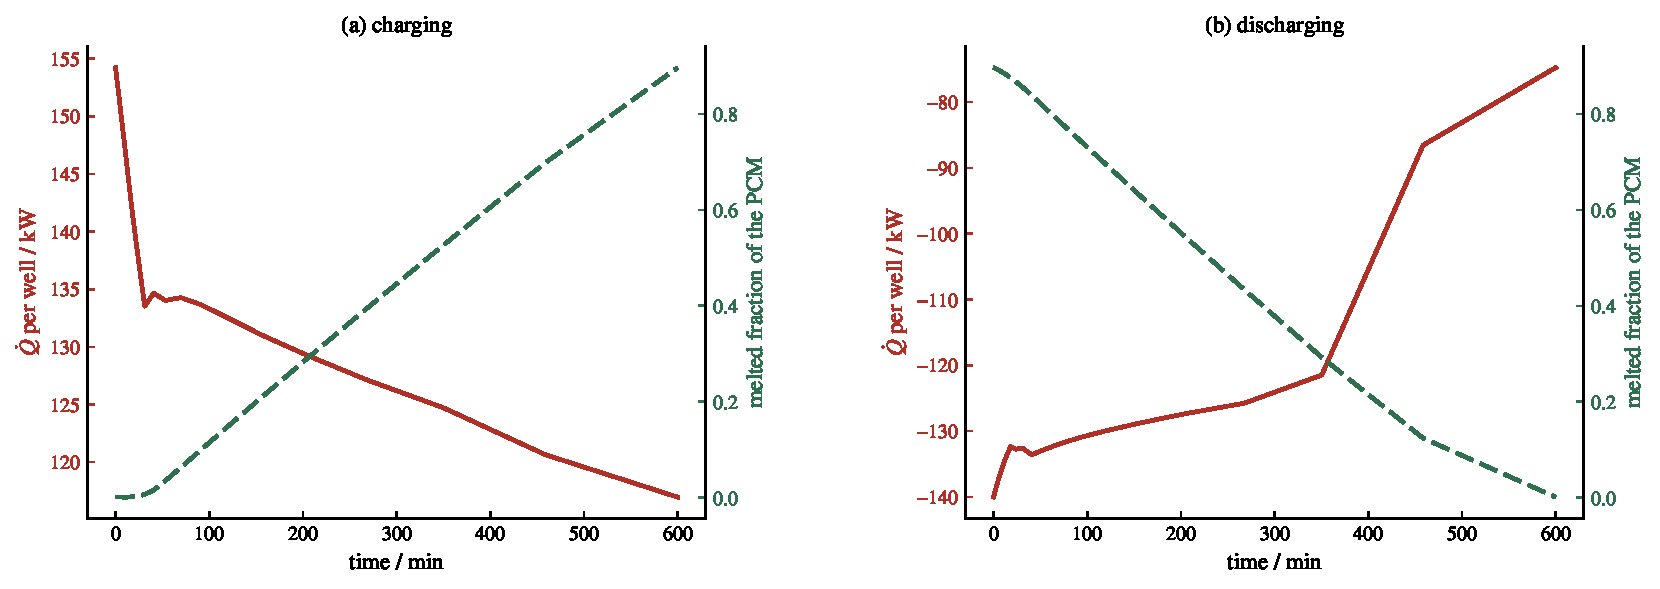
\includegraphics[width=\linewidth]{figures/BOREAS_prof_integrals.pdf}
\caption{Heat transfer rate integrated along the well, per storage well, and
the fraction of the PCM inventory that has changed phase, against time from
the start of each half-cycle.}
\label{fig:prof-int}
\end{figure}
